\documentclass{beamer}
\usepackage[utf8]{inputenc}
\usepackage{listings}
\usepackage{booktabs}
\usepackage{nicefrac}
\usepackage{amssymb}
\usepackage{amsmath}
\usepackage{bm}
\usepackage{enumitem}
\usepackage{hyperref}
\usepackage[export]{adjustbox}
\usepackage{svg}

\usetheme{Madrid}
\definecolor{mlpblue}{rgb}{0.1, 0.14, 0.24}

\useoutertheme{infolines} % Alternatively: miniframes, infolines, split
\useinnertheme{circles}
\usecolortheme[named=mlpblue]{structure}

\lstset{basicstyle=\footnotesize\ttfamily,breaklines=true}

%------------------------------------------------------------
%This block of code defines the information to appear in the
%Title page
\title[Mechanistic Interpretability]{A Practical Guide to Mechanistic Interpretability:}

\subtitle{Demistifying black boxes with \textbf{Sparse AutoEncoders}\thanks{\tiny \url{https://transformer-circuits.pub/2023/monosemantic-features/}}\thanks{\tiny \url{https://arxiv.org/abs/2404.16014}}\thanks{\tiny{\url{https://www.arena.education/}}}}

\author[Machine Learning @ Purdue] % optional
{J.~Setpal} 

\date{\today}

\titlegraphic{
\includegraphics[width=7cm]{../shared/logo-long.pdf}}

%End of title page configuration block
%------------------------------------------------------------

%The next block of commands puts the table of contents at the 
%beginning of each section and highlights the current section:

\AtBeginSection[]
{
  \begin{frame}
    \frametitle{Outline}
    \tableofcontents[currentsection]
  \end{frame}
}
% ------------------------------------------------------------


\begin{document}

\frame{\titlepage}


%---------------------------------------------------------
% This block of code is for the table of contents after
% the title page
\begin{frame}
\frametitle{Outline}
\tableofcontents
\end{frame}
%---------------------------------------------------------

\section{Background \& Intuition}
\begin{frame}{What is Interpretability?}
	\begin{columns}
		\begin{column}{0.5\textwidth}
			\begin{center}
				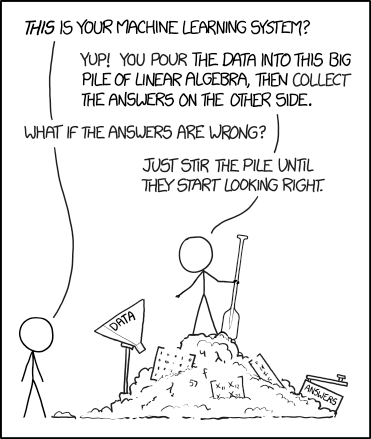
\includegraphics[width=5cm]{img/1838} \pause
			\end{center}
		\end{column}
		\begin{column}{0.5\textwidth}
			Interpretability within Machine Learning is the \textbf{degree} to which we can understand the \textbf{cause} of a decision, and use it to consistently \underline{predict the model's prediction}. \pause \newline \\

			This is easy for shallow learning. \pause For deep learning however, it is a \textbf{lot harder}. \pause \newline \\
			Today, we will interpret deep neural networks (transformers). 
		\end{column}
	\end{columns}
\end{frame}

\begin{frame}{What is \textit{Mechanistic} Interpretability?}
	Most of interpretability seeks to extract representations from weights:
	
	\begin{center}
		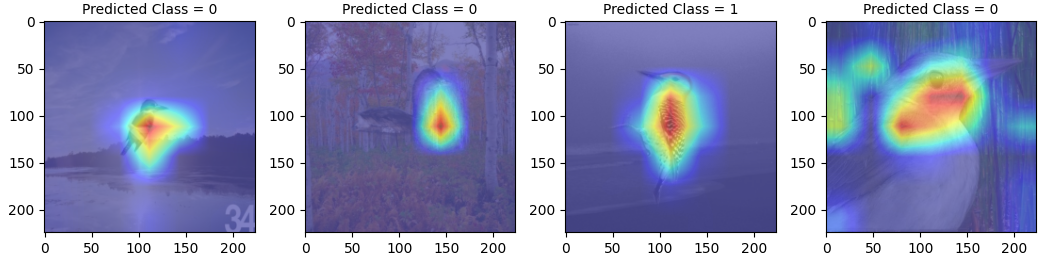
\includegraphics[width=\textwidth]{img/cams}
	\end{center} \pause

	Mechanistic Interpretability is a subset of interpretability, that places a focus on \textbf{reverse engineering neural networks}. \pause \newline \\

	It seeks to understand functions that \textit{individual neurons} play in the inference of a neural network. \pause \newline \\
	
	This can subsequently be used to offer high-level explanations for decisions, as well as guarantees during inference.
\end{frame}

\section{Sparse AutoEncoders}
\begin{frame}{Transformers Mini-Review}
	\textbf{Crucial Aside:} Treat residual connections as ``memory''; all other layers ``read from'', ``process'', and ``write-to'' memory! \pause
	\begin{center}
		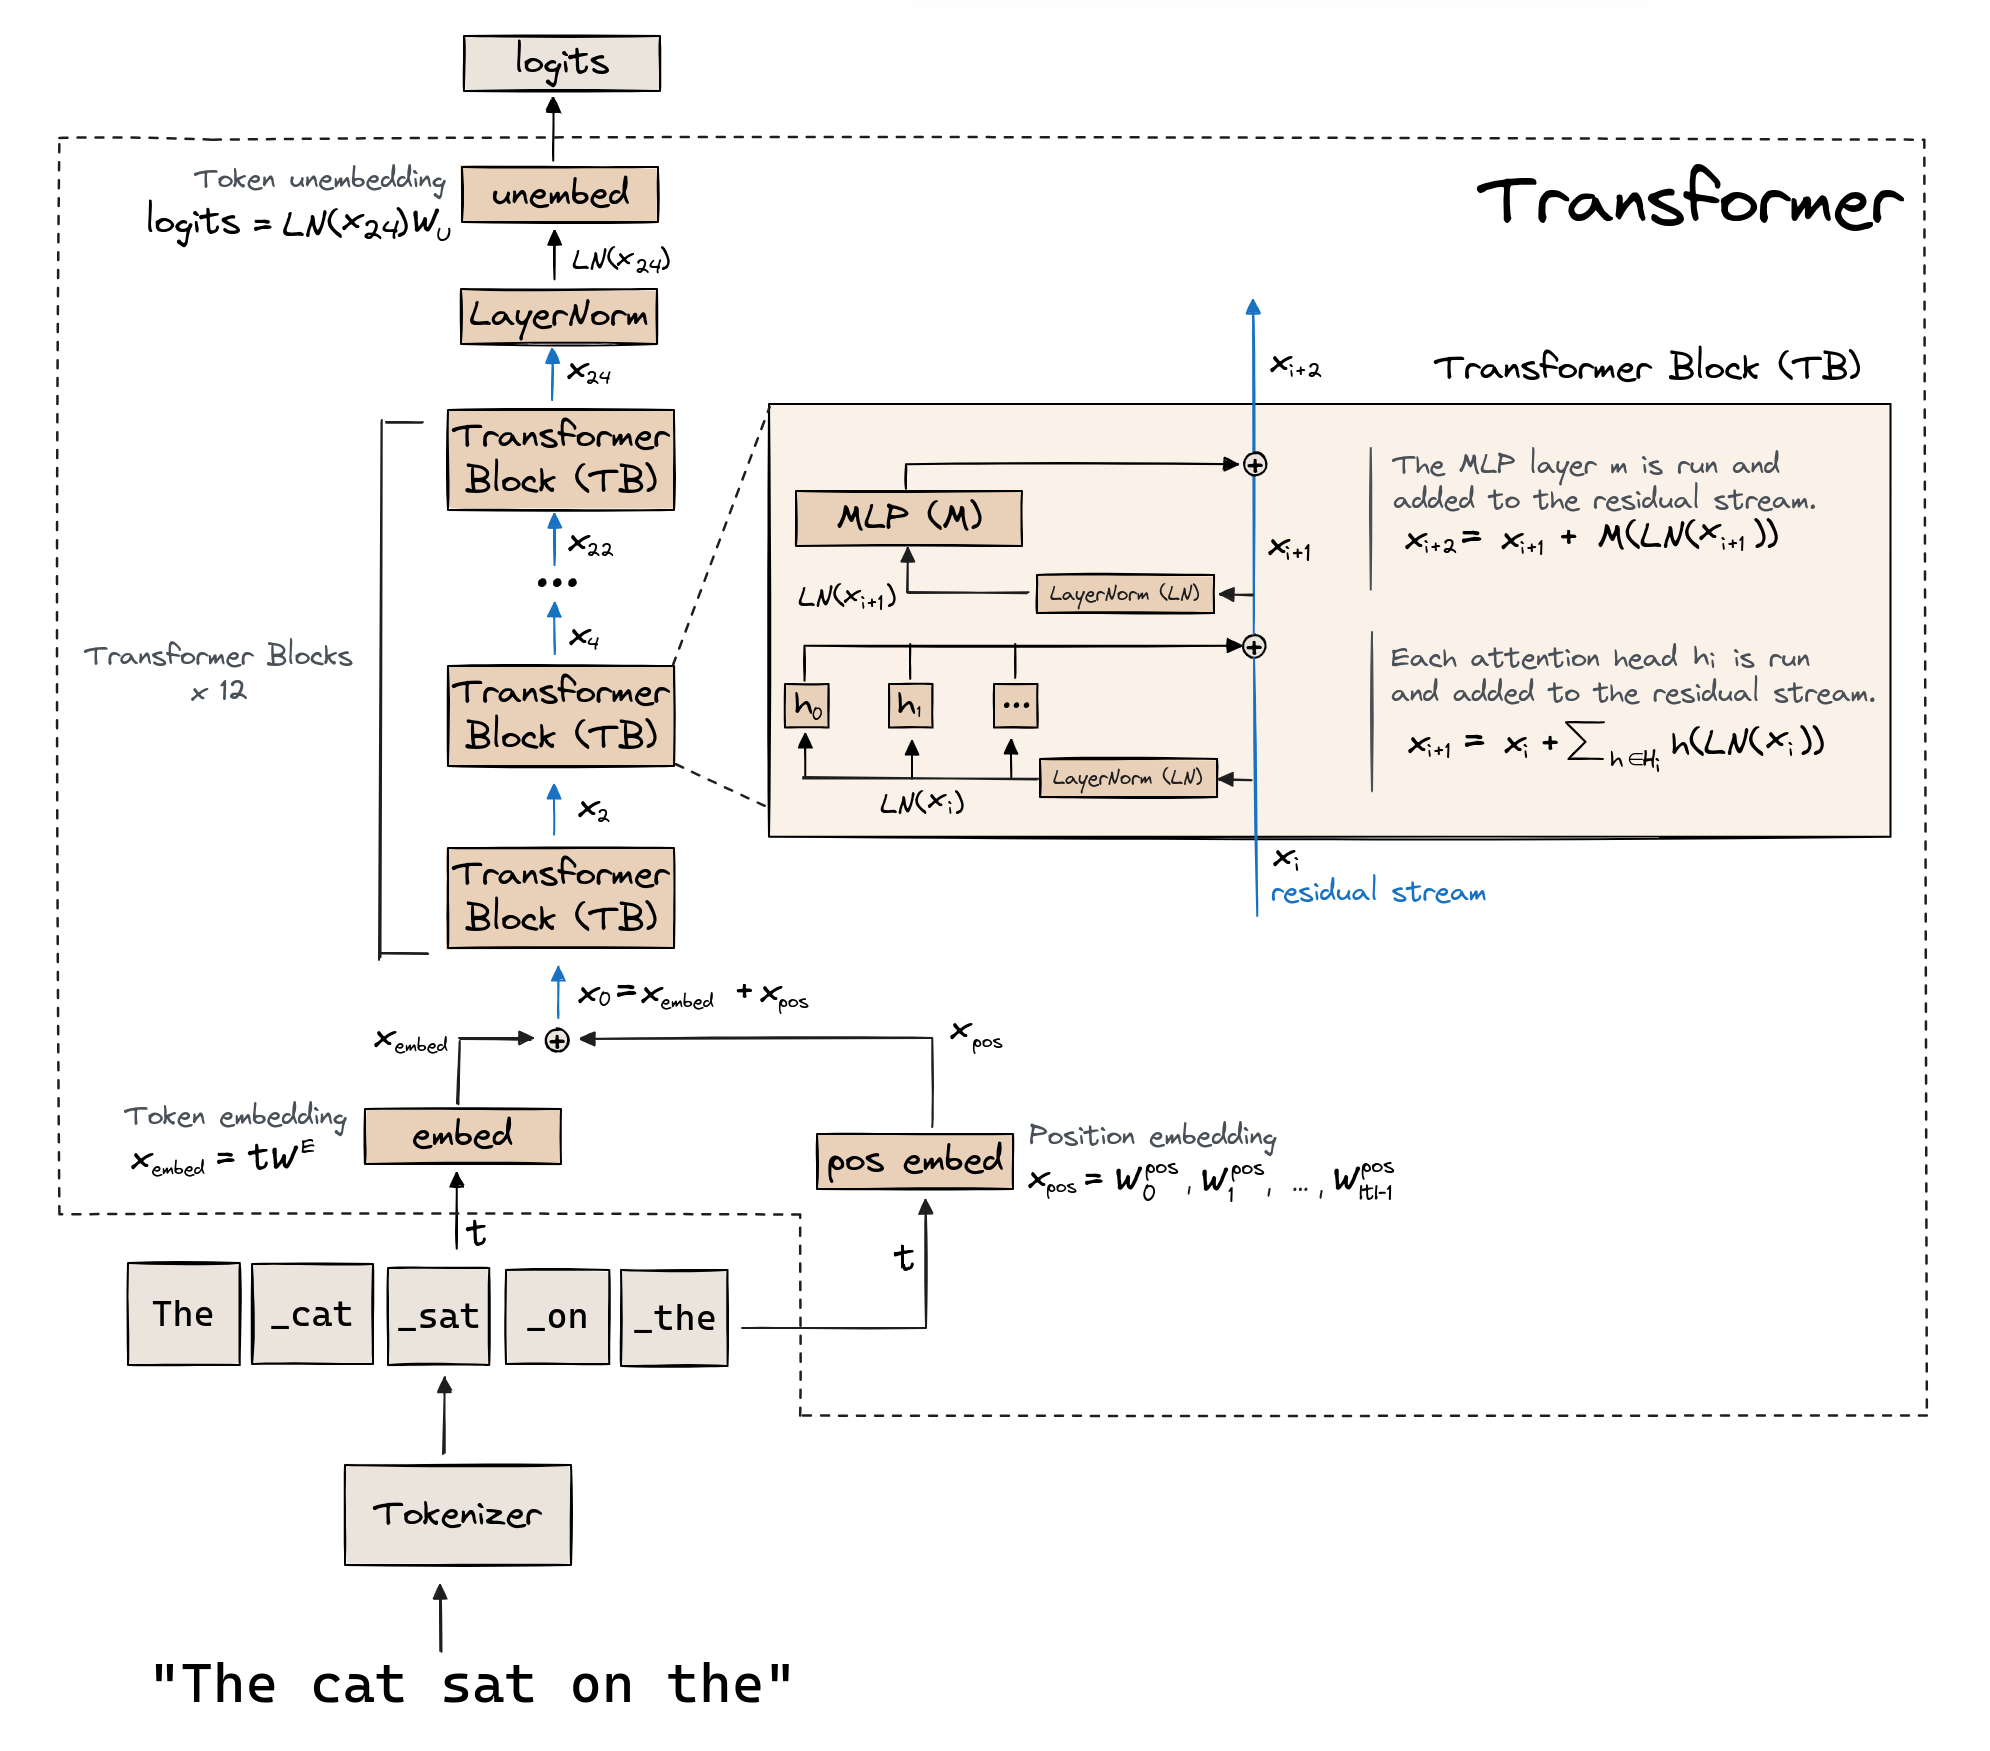
\includegraphics[width=.65\textwidth]{img/transformer.png}
	\end{center}
\end{frame}

\begin{frame}{Problem Setup}
	\textbf{Q:} Now, given the framework we just discussed, what stops from directly analyzing MLP activations? \pause \\
	\textbf{A:} Enter \textbf{polysemanticity} \& \textbf{superposition}. \pause

	\begin{columns}
		\begin{column}{.44\textwidth}
			\begin{center}
				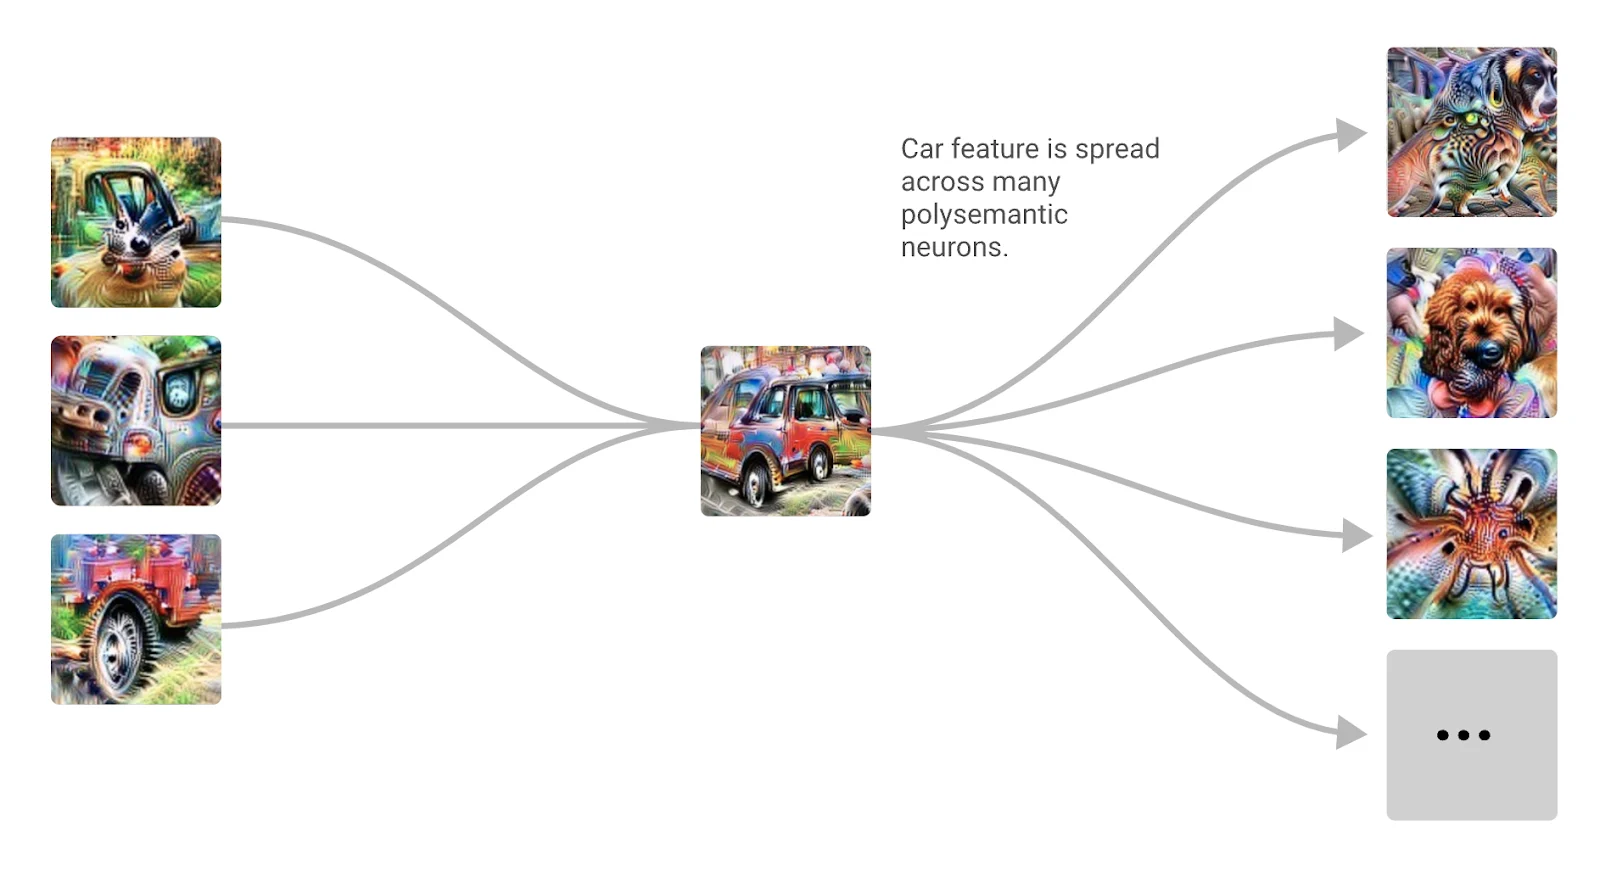
\includegraphics[width=\textwidth]{img/polysemanticity.png}
			\end{center}
			When we perform an indvidual analysis of neurons, we observe it \underline{fires for unrelated concepts}. \newline \\

			This is \textbf{polysemanticity}. \pause
		\end{column}
		\begin{column}{.5\textwidth}
			\begin{center}
				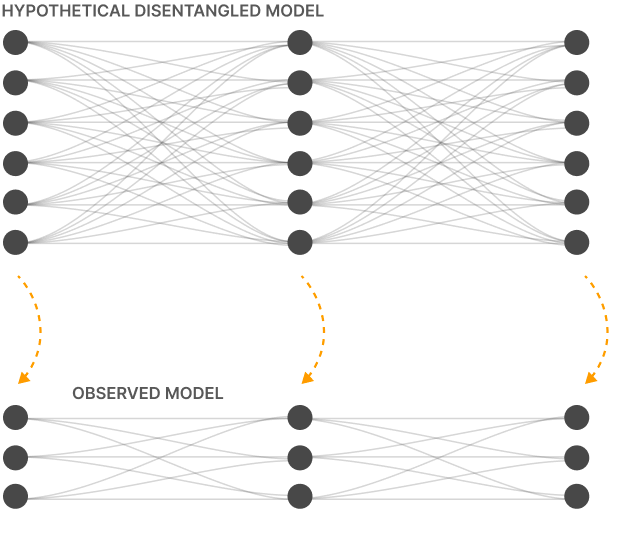
\includegraphics[width=.6\textwidth]{img/superposition.png}
			\end{center}
			We observe learning compresses larger models to smaller footprints \underline{using denser parameters}. \newline \\
			This is \textbf{superposition}.
		\end{column}
	\end{columns}
\end{frame}

\begin{frame}{Analytical Setup}
	We will explore the following setup:
	\begin{center}
		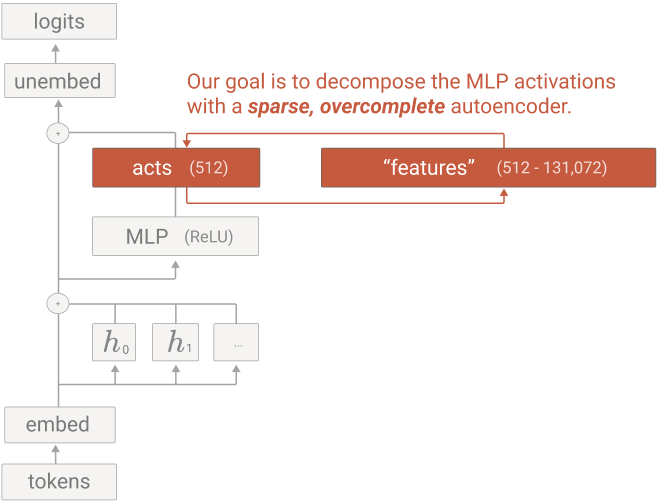
\includegraphics[width=.6\textwidth]{img/mono-arch.png}
	\end{center}
\end{frame}

\begin{frame}{Training Setup}
	\vspace{-2em}
	\begin{table}[t]
		\begin{center}
			\hspace*{-0.75em}
			\begin{tabular}{l|cc}
				\toprule
				& \bf Transformer & \bf Sparse Autoencoder \\
				\midrule
				\bf Layers & \begin{tabular}{@{}c@{}} 1 Attention Block \\ 1 MLP Block \end{tabular} & \begin{tabular}{@{}c@{}} 1 ReLU \\ 1 Linear \end{tabular} \\
					\bf MLP Size & $512$ & $512 \times f \in \{1, \ldots, 256\}\footnote{$f=8$ for our analysis}$ \\
				\bf Dataset & The Pile (100B tokens) & Activations (8B samples) \\
				\bf Loss & Autoregressive Log-Likelihood & \begin{tabular}{@{}c@{}} $L2$ Reconstruction  \\ $L1$ on hidden-layer activation \end{tabular} \\
				\bottomrule
			\end{tabular}
		\end{center}
	\end{table} \pause
	\underline{Objective:} \textit{polysemantic activations} $\stackrel{Tr~}{\rightarrow}$ \textbf{monosemantic features}. \pause \newline \\

	The sparse, overcomplete autoencoder is trained against this objective.
	\begin{enumerate}[label=\arabic*.]
		\item \textbf{Sparse} because we constrain activations (L1 penalty).
		\item \textbf{Overcomplete} because the hidden layer exceeds the input dimension.
	\end{enumerate}
\end{frame}

\begin{frame}{Sparse Dictionary Learning}
	Given $X := \{x^j\}^K_{j=1}; x_i \in \mathbb{R}^d$, we wish to find $D \in \mathbb{R}^{d \times n}, R \in \mathbb{R}^n$ s.t:
	\begin{gather}
		||X-DR||^2_F \approx 0
	\end{gather} \pause
	We can motivate our objective transformation by linear factorization:
	\begin{gather}
		x^j \approx b_D + \sum_i f_i(x^j)d_i \\
		f_i = \sigma_{ReLU}(W_E(x-b_D)+ b_E)
	\end{gather}
	where $d_i$ is the `feature direction' represented as columns of the $W_D$. \pause \newline \\
	
	Some interesting implementation notes:
	\begin{enumerate}[label=\alph*.]
		\item Training data $\propto n($interpretable features$)$. \pause
		\item Tying $b_D$ before the encoder and after the decoder \underline{improves performance}. \pause
		\item Dead neurons are periodically \textit{resampled} to improve feature representations.
	\end{enumerate}
\end{frame}

\begin{frame}{Evaluating Interpretability}
	Reliable evaluations on interpretability were scored based on a rubric:
	\begin{center}
		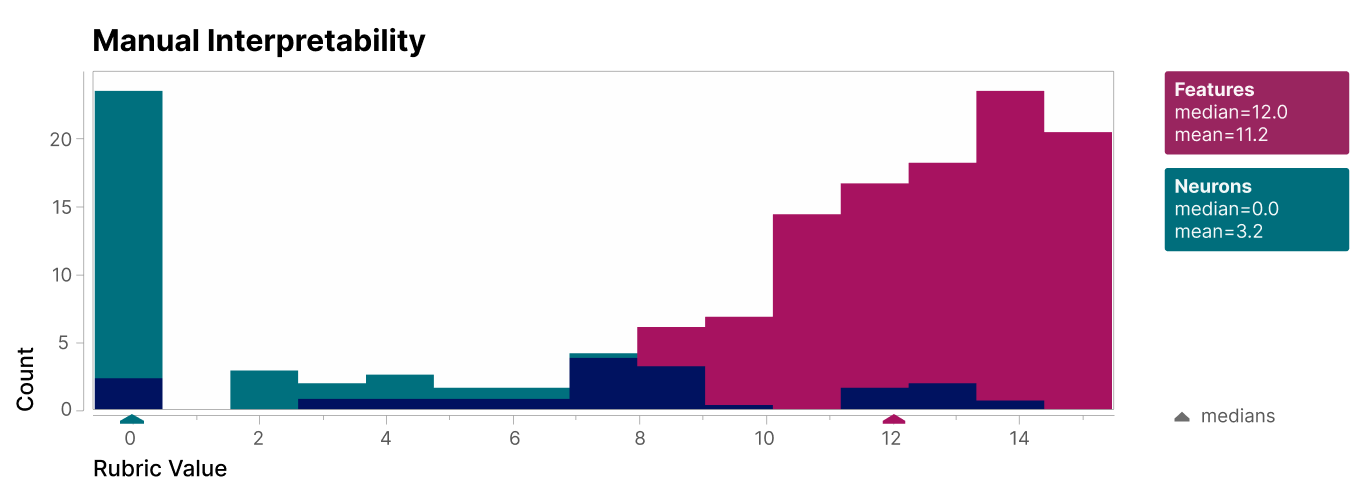
\includegraphics[width=.7\textwidth]{img/scores.png}
		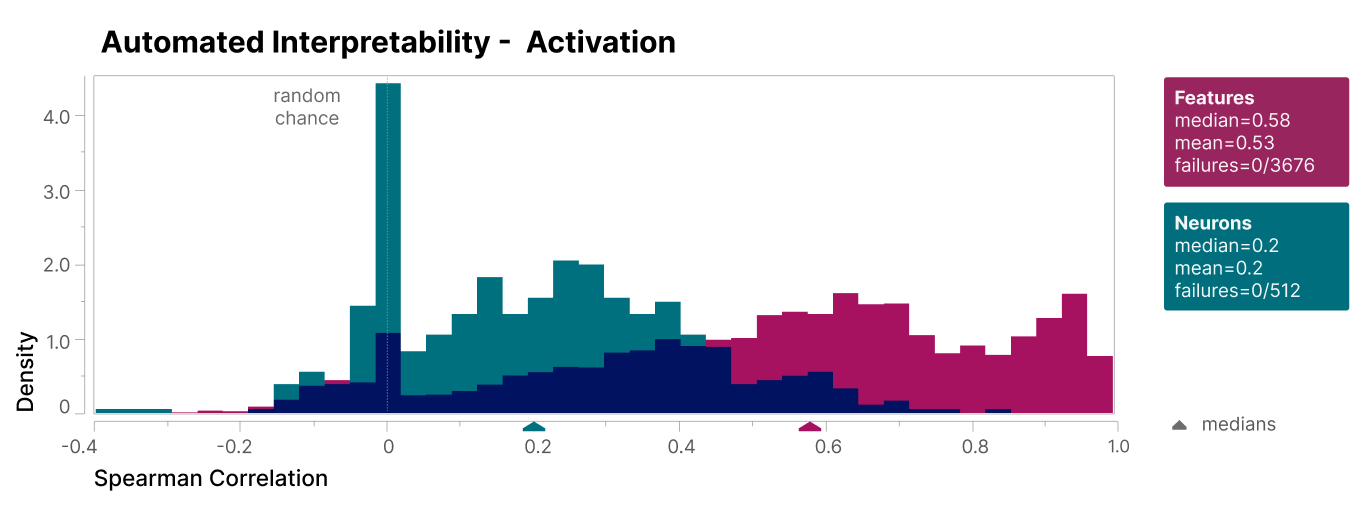
\includegraphics[width=.7\textwidth]{img/ascores-activ.png}
	\end{center}
	\vspace{-1em}
	Features were found to be interpretable when score $> 8$.
\end{frame}

\begin{frame}{Analyzing Arabic Features}
	Let's analyze feature \textbf{A/1/3450}, that fires on \underline{Arabic Script}. \pause

	\begin{block}{}
		This is effectively \textit{invisible} when viewed through the polysemantic model!
	\end{block} \pause
	We can evaluate each token using the log-likelihood ratio:
	\begin{gather}
		LL(t) = \log{(P(t|\text{Arabic})/P(t))}
	\end{gather}
	\begin{columns}
		\begin{column}{.3\textwidth}
			Despite representing $0.13\%$ of training data, arabic script makes up $\bm{81\%}$ \textbf{of active tokens}:
		\end{column}
		\begin{column}{.7\textwidth}
			\vspace{-2.5em}
			\begin{center}
				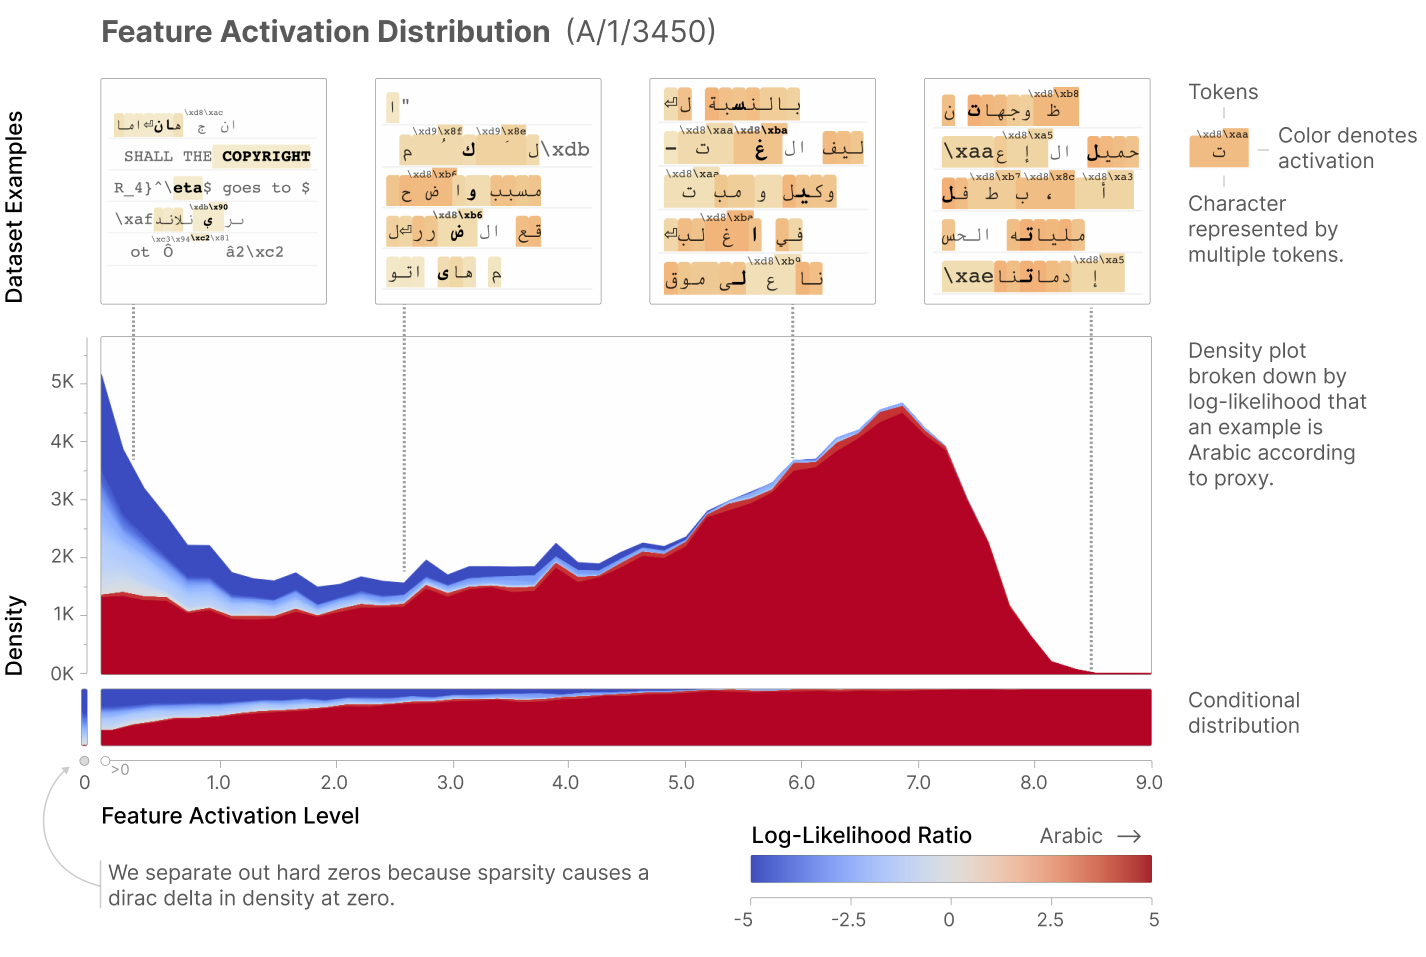
\includegraphics[width=.9\textwidth]{img/arabic.png}
			\end{center}
		\end{column}
	\end{columns}
\end{frame}

\begin{frame}{Pinned Feature Sampling}
	They can be used to steer generation.
	\begin{center}
		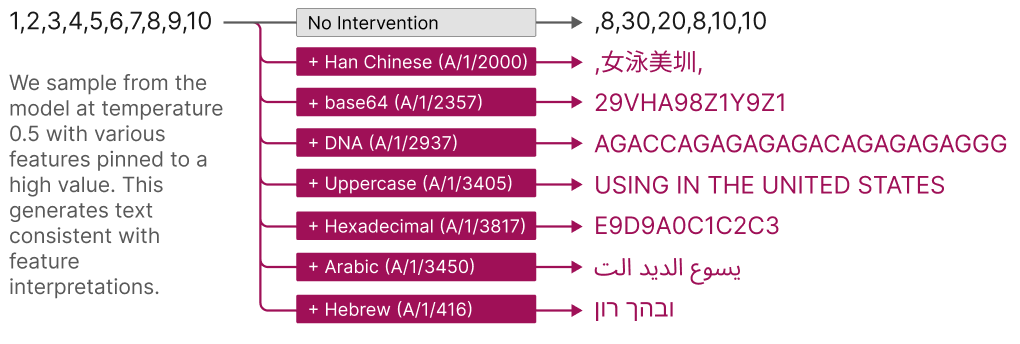
\includegraphics[width=.7\textwidth]{img/sampling.png}
	\end{center} \pause

	\textbf{Approach:} Set high values of features demonstrating desired behaviors, and then sample from the model. \pause \newline \\

	We observe that \underline{interpreted features are actively used by the model}.
\end{frame}

\begin{frame}{Finite State Automaton}
	A unique feature of features is their role as \textbf{finite state automaton}. \pause \newline \\

	Unlike circuits, these work by \underline{daisy chaining features} that increase the probability of another feature firing in a loop-like fashion. \pause \newline \\

	These present partial explanations of \textbf{memorizations} within transformers:
	\begin{center}
		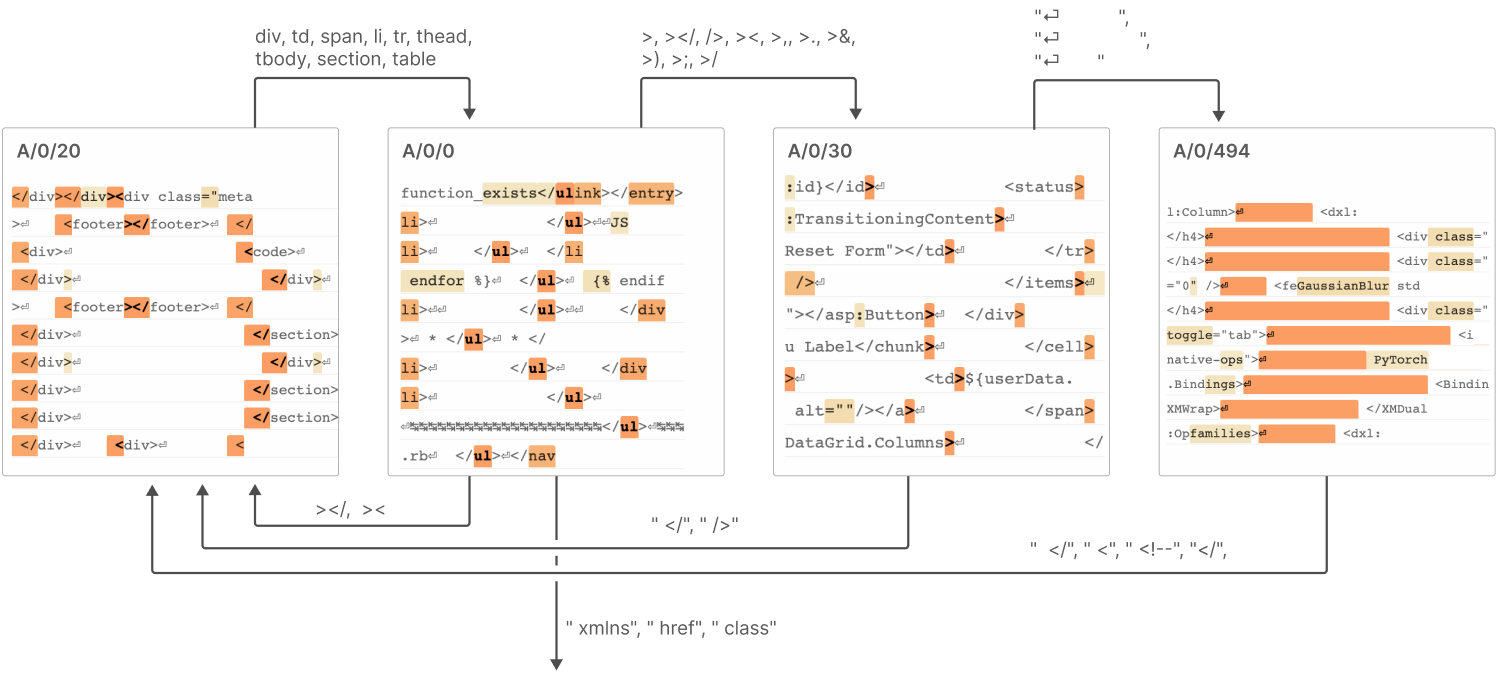
\includegraphics[width=.8\textwidth]{img/fsa.png}
	\end{center}
\end{frame}

\begin{frame}{Modern (Gated) SAEs ($\nicefrac{1}{2}$)}
	Quick review of the structure of the original SAE:
	\begin{align}
		f(x) &:= \sigma_{\text{ReLU}}(W_E (x - b_D) + b_E) \\
		\hat{x}(f(x)) &:= W_D f(x) + b_D \\
		\min_{W_E, W_D, b_D, b_e} \mathcal{L}(x) &= \min_{W_E, W_D, b_D, b_e} \underbrace{\| x - \hat{x}(f(x)) \|^2_2}_{\text{reconstruction error}} + \underbrace{\lambda \| f(x) \|_1}_{\text{sparsity penalty}}
	\end{align} \pause
	We evaluate the SAE by how much loss increases when \textbf{activations are substituted with the reconstructions} during forward pass. \pause \newline \\

	\textbf{Observation:} $\| \cdot \|_1$ motivates \textit{shrinkage} -- minimizing sparsity is ``easier'' than reconstructing sparse features, and motivates under-activation of reconstructed features.
\end{frame}

\begin{frame}{Modern (Gated) SAEs ($\nicefrac{2}{2}$)}
	\textbf{Idea:} Let's disentangle feature importance with feature existance:
	\begin{center}
		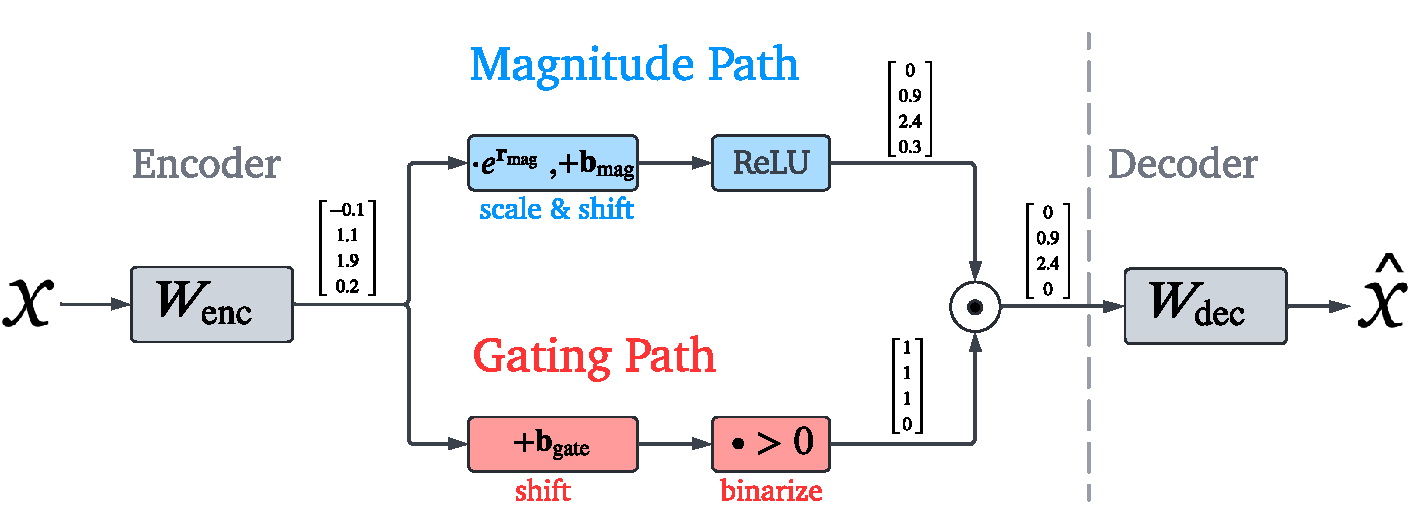
\includegraphics[width=.85\textwidth]{img/gated-sae.pdf}
	\end{center} \pause
	\vspace{-1em}

	For this, the authors also define the following loss function:
	\begin{gather*}
		\mathcal{L}(x) := \|x - \hat{x}(f(x)) \|^2_2 + \underbrace{\lambda \| \sigma_{\text{ReLU}} (f_{g}(x)) \|_1}_{f_g := \text{ pre-activation}} + \| x - \hat{x}(\sigma_{\text{ReLU}}(f_g(x))) \|^2_2
	\end{gather*} \pause
	Finally, they also use weight-tying to reduce parameter explosion.
\end{frame}

\section{Applications \& Practical Detail}
\begin{frame}{Training SAEs}
	\begin{center}
		If you can view this screen, I am making a mistake.
	\end{center}
\end{frame}

\begin{frame}{Dashboard Interpretation}
	\begin{center}
		If you can view this screen, I am making a mistake.
	\end{center}
\end{frame}

\begin{frame}{Feature Steering with SAEs}
	\begin{center}
		If you can view this screen, I am making a mistake.
	\end{center}
\end{frame}

\begin{frame}{Thank you!}
	\begin{center}
		Have an awesome rest of your day!
	\end{center}
	\begin{center}
		\textbf{Slides:} \url{https://jinen.setpal.net/slides/sae.pdf}
	\end{center}
\end{frame}

\end{document}
